\chapter{第4套试卷——参考答案与评分标准}

% 加载TikZ扩展库（用于状态图和框图）
\usetikzlibrary{automata, positioning, arrows}

%=============================================================================
\section*{一、选择题参考答案（每题3分，共18分）}
%=============================================================================

\begin{framed}
\textbf{评分标准：}每题3分，选择正确得3分，错误或不选得0分。本题共6题，满分18分。
\end{framed}

\begin{enumerate}[label=\arabic*.]
\item \textbf{答案：C（PAL）}

\textbf{解析：}PAL（Programmable Array Logic）的典型结构是与阵列可编程、或阵列固定。GAL在PAL基础上增加了输出逻辑宏单元（OLMC），但基本原理相同。CPLD基于乘积项结构，FPGA基于查找表结构。

\item \textbf{答案：B（定义电路的输入输出端口）}

\textbf{解析：}ENTITY（实体）是VHDL设计的基本单元，其核心作用是对外定义电路的输入输出端口（PORT）。内部逻辑功能由ARCHITECTURE（结构体）描述；信号在ARCHITECTURE内部声明；仿真激励由Testbench提供。

\item \textbf{答案：C（SRAM存储单元和译码器）}

\textbf{解析：}FPGA中查找表（LUT）的本质是一个小容量SRAM加上译码电路。$n$输入LUT中有$2^n$个SRAM存储单元，输入信号经译码器选择对应的SRAM单元输出。上电时从外部配置存储器加载真值表到SRAM中。

\item \textbf{答案：B（信号赋值在当前进程结束时才更新，进程内读到的是旧值）}

\textbf{解析：}VHDL中SIGNAL的赋值（使用\texttt{<=}）具有$\delta$延时特性：在一个PROCESS内部，所有信号赋值语句都要等到进程执行完毕（挂起）后才统一更新。在进程内读取信号将得到更新前的旧值。与之相对，VARIABLE的赋值（使用\texttt{:=}）立即生效。

\item \textbf{答案：B（4）}

\textbf{解析：}$n$输入LUT可以实现的任意组合逻辑函数的最大输入变量数为$n$。4输入LUT有$2^4=16$个配置位，可表示任意4变量逻辑函数的完整真值表。实现更多变量需多个LUT级联。

\item \textbf{答案：A（一个查找表和一个触发器）}

\textbf{解析：}典型FPGA的逻辑单元（Logic Element, LE）通常包含一个$n$输入LUT（实现组合逻辑）和一个D触发器（实现时序逻辑），外加一些选择器和进位链。乘法器、RAM块、处理器核等属于FPGA中的专用硬核资源，不在基本逻辑单元中。

\end{enumerate}

%=============================================================================
\section*{二、填空题参考答案（每题3分，共12分）}
%=============================================================================

\begin{framed}
\textbf{评分标准：}每空1.5分（每道题含两空时每空各1.5分，含一空时该空3分），答对得满分，拼写错误酌情扣0.5分。本题共4题，满分12分。
\end{framed}

\begin{enumerate}[label=\arabic*.]

\item \textbf{答案：SIGNAL；CONSTANT}

\textbf{解析：}VHDL中\texttt{SIGNAL}关键字用于声明电路内部互连信号（相当于物理连线），具有$\delta$延时特性；\texttt{CONSTANT}关键字用于声明常量，其值在编译时确定且不可更改。

\item \textbf{答案：std\_logic\_1164}

\textbf{解析：}\texttt{ieee.std\_logic\_1164}是IEEE标准库中最核心的程序包，定义了9值逻辑类型\texttt{STD\_LOGIC}（包括\texttt{'U'}, \texttt{'X'}, \texttt{'0'}, \texttt{'1'}, \texttt{'Z'}, \texttt{'W'}, \texttt{'L'}, \texttt{'H'}, \texttt{'-'}）以及其向量\texttt{STD\_LOGIC\_VECTOR}。

\item \textbf{答案：WHEN-ELSE；WITH-SELECT-WHEN}

\textbf{解析：}VHDL并行信号赋值语句的三种形式：
\begin{itemize}
  \item 简单信号赋值：\texttt{y <= a AND b;}
  \item 条件信号赋值：\texttt{y <= a WHEN sel='0' ELSE b;}（WHEN-ELSE形式）
  \item 选择信号赋值：\texttt{WITH sel SELECT y <= a WHEN '0', b WHEN '1';}（WITH-SELECT-WHEN形式）
\end{itemize}
三者均为并行语句，放置在结构体的BEGIN-END之间，不在PROCESS内。

\item \textbf{答案：Complex；与（AND）}

\textbf{解析：}CPLD全称为Complex Programmable Logic Device（复杂可编程逻辑器件）。其内部结构主要由可编程的\textbf{与阵列}和\textbf{宏单元（Macrocell）}组成。宏单元通常包含一个或门、一个触发器和输出选择电路。CPLD基于乘积项结构，与FPGA的查找表结构不同。

\end{enumerate}

%=============================================================================
\section*{三、程序改错题参考答案（共5分）}
%=============================================================================

\begin{framed}
\textbf{评分标准：}找出并正确改正5处错误即得满分5分（每题1分）。若找出全部6处，仍按5分计。仅指出错误位置但未说明改正方法者，每处扣0.5分。
\end{framed}

以下逐行列出6处错误：

\begin{enumerate}[label=\textbf{错误\arabic*：}]

\item \textbf{第1行：\texttt{library ieee} 缺少分号}

\textbf{改正：}在行末添加分号，即 \texttt{library ieee;}

\item \textbf{第2行：\texttt{use ieee.std\_logic\_1164.all} 缺少分号}

\textbf{改正：}在行末添加分号，即 \texttt{use ieee.std\_logic\_1164.all;}

\item \textbf{第10行：变量声明缺少分号}

\textbf{改正：}在变量声明行末添加分号，即：
\begin{lstlisting}
variable temp : std_logic_vector(3 downto 0);
\end{lstlisting}

\item \textbf{第9行：PROCESS敏感信号表不完整}

\textbf{改正：}敏感信号表中缺少\texttt{d0, d1, d2, d3}。当这些输入信号变化时，进程也需要重新执行。应改为：
\begin{lstlisting}
process(d0, d1, d2, d3, sel)
\end{lstlisting}

\noindent 或使用\texttt{process(all)}（VHDL-2008）自动包含所有读取的信号。

\item \textbf{第13--18行：变量\texttt{temp}使用了信号赋值符号\texttt{<=}}

\textbf{改正：}VHDL中变量的赋值符号为\texttt{:=}，而非\texttt{<=}。应将5处赋值语句中的\texttt{<=}全部改为\texttt{:=}：
\begin{lstlisting}
when "00" => temp := d0;
when "01" => temp := d1;
when "10" => temp := d2;
when "11" => temp := d3;
when others => temp := (others => '0');
\end{lstlisting}

\item \textbf{第20行：输出端口\texttt{y}使用了变量赋值符号\texttt{:=}}

\textbf{改正：}\texttt{y}是\texttt{OUT}端口信号，必须使用信号赋值符号\texttt{<=}。应改为：
\begin{lstlisting}
y <= temp;
\end{lstlisting}

\end{enumerate}

\noindent\textbf{修正后的完整正确代码：}
\begin{lstlisting}[caption={修正后的4选1多路选择器}, label={lst:ans04_correct}]
library ieee;
use ieee.std_logic_1164.all;

entity mux4to1 is
  port (
    d0, d1, d2, d3 : in  std_logic_vector(3 downto 0);
    sel            : in  std_logic_vector(1 downto 0);
    y              : out std_logic_vector(3 downto 0)
  );
end mux4to1;

architecture behavioral of mux4to1 is
begin
  process(d0, d1, d2, d3, sel)
    variable temp : std_logic_vector(3 downto 0);
  begin
    case sel is
      when "00"   => temp := d0;
      when "01"   => temp := d1;
      when "10"   => temp := d2;
      when "11"   => temp := d3;
      when others => temp := (others => '0');
    end case;
    y <= temp;
  end process;
end behavioral;
\end{lstlisting}

%=============================================================================
\section*{四、程序阅读分析题参考答案（共5分）}
%=============================================================================

\begin{framed}
\textbf{评分标准：}第（1）问2分，功能描述正确得2分，部分正确得1分；第（2）问3分，判断正确得1分，依据充分得2分（每条依据1分）。本题共5分。
\end{framed}

\begin{enumerate}[label=(\arabic*)]

\item \textbf{该电路实现的功能（2分）：}

该电路是一个\textbf{4输入优先级编码器}（4-to-2 Priority Encoder）。

输入\texttt{din[3:0]}（4位），输出\texttt{dout[1:0]}（2位编码值）和\texttt{v}（有效标志）。

优先级规则：\texttt{din(3)}优先级最高，\texttt{din(0)}优先级最低。即：
\begin{itemize}
  \item 若 \texttt{din(3)='1'}，则输出 \texttt{dout="11"}（编码3），\texttt{v='1'}
  \item 若 \texttt{din(3)='0'} 且 \texttt{din(2)='1'}，则输出 \texttt{dout="10"}（编码2），\texttt{v='1'}
  \item 若 \texttt{din[3:2]="00"} 且 \texttt{din(1)='1'}，则输出 \texttt{dout="01"}（编码1），\texttt{v='1'}
  \item 若 \texttt{din[3:1]="000"} 且 \texttt{din(0)='1'}，则输出 \texttt{dout="00"}（编码0），\texttt{v='1'}
  \item 若 \texttt{din="0000"}，则输出 \texttt{dout="00"}，\texttt{v='0'}（无效）
\end{itemize}

\item \textbf{是组合逻辑还是时序逻辑？判断依据（3分）：}

\textbf{答：该电路是组合逻辑电路。}

判断依据如下：
\begin{enumerate}
  \item \textbf{无时钟信号（1.5分）：}代码中没有\texttt{clk}信号，也没有使用\texttt{if rising\_edge(clk)}或\texttt{wait until}等边沿检测语句。时序逻辑必须有时钟信号。
  \item \textbf{敏感信号表仅包含输入信号（1.5分）：}PROCESS的敏感信号表为\texttt{(din)}，仅包含所有输入信号。当且仅当输入信号变化时进程才会被触发，输出随输入即时更新。进程内所有输出信号（\texttt{dout}, \texttt{v}）在每次执行时均被赋值，不会产生锁存。
\end{enumerate}

\end{enumerate}

%=============================================================================
\section*{五、综合设计题参考答案（共60分）}
%=============================================================================

%-----------------------------------------------------------------------------
\subsection*{设计题1：8位二进制比较器（20分）}
%-----------------------------------------------------------------------------

\begin{framed}
\textbf{评分标准：}
\begin{itemize}
  \item 端口框图（5分）：框图和接口标注正确清晰得5分；缺少位宽标注或信号遗漏扣1--2分。
  \item VHDL代码（10分）：实体定义正确3分，结构体逻辑正确5分，代码规范（缩进、注释）2分。
  \item Testbench（5分）：覆盖A>B、A=B、A<B三种情况各1.5分，代码完整规范0.5分。
\end{itemize}
\end{framed}

\subsubsection*{(1) 顶层模块端口框图（5分）}

\begin{center}
\begin{tikzpicture}[
  block/.style={rectangle, draw=black, thick, minimum width=5cm, minimum height=3.5cm,
                align=center, fill=blue!10},
  port/.style={font=\ttfamily\footnotesize}
]

\node[block] (comp) at (0,0) {
  \textbf{comparator\_8bit}\\[0.3cm]
  8位二进制比较器
};

% Input A
\draw[<-] (-4.5, 1.2) -- (-2.5, 1.2)
  node[pos=0, left, port] {A[7:0]};

% Input B
\draw[<-] (-4.5, 0.4) -- (-2.5, 0.4)
  node[pos=0, left, port] {B[7:0]};

% Output AGTBOUT
\draw[->] (2.5, 1.2) -- (4.5, 1.2)
  node[pos=1, right, port] {AGTBOUT};

% Output AEQBOUT
\draw[->] (2.5, 0.4) -- (4.5, 0.4)
  node[pos=1, right, port] {AEQBOUT};

% Output ALTBOUT
\draw[->] (2.5, -0.4) -- (4.5, -0.4)
  node[pos=1, right, port] {ALTBOUT};

\end{tikzpicture}
\end{center}

\noindent\textbf{端口说明：}
\begin{itemize}
  \item \texttt{A[7:0]}：8位输入，被比较数A
  \item \texttt{B[7:0]}：8位输入，被比较数B
  \item \texttt{AGTBOUT}：1位输出，A > B时为\texttt{'1'}，否则为\texttt{'0'}
  \item \texttt{AEQBOUT}：1位输出，A = B时为\texttt{'1'}，否则为\texttt{'0'}
  \item \texttt{ALTBOUT}：1位输出，A < B时为\texttt{'1'}，否则为\texttt{'0'}
\end{itemize}

\subsubsection*{(2) 完整VHDL代码（10分）}

\begin{lstlisting}[caption={8位二进制比较器——完整VHDL代码}, label={lst:ans04_comp}]
library ieee;
use ieee.std_logic_1164.all;
use ieee.numeric_std.all;   -- 使用 numeric_std 进行算术比较

entity comparator_8bit is
  port (
    A       : in  std_logic_vector(7 downto 0);  -- 8位输入A
    B       : in  std_logic_vector(7 downto 0);  -- 8位输入B
    AGTBOUT : out std_logic;                     -- A>B 标志
    AEQBOUT : out std_logic;                     -- A=B 标志
    ALTBOUT : out std_logic                      -- A<B 标志
  );
end comparator_8bit;

architecture behavioral of comparator_8bit is
begin
  -- 比较过程：使用IF-ELSE实现优先级判断
  process(A, B)
  begin
    -- 默认值，防止锁存
    AGTBOUT <= '0';
    AEQBOUT <= '0';
    ALTBOUT <= '0';

    if unsigned(A) > unsigned(B) then
      AGTBOUT <= '1';
    elsif unsigned(A) = unsigned(B) then
      AEQBOUT <= '1';
    else
      ALTBOUT <= '1';
    end if;
  end process;
end behavioral;
\end{lstlisting}

\noindent\textbf{代码说明：}
\begin{itemize}
  \item 使用\texttt{ieee.numeric\_std.all}库中的\texttt{unsigned()}类型转换，将\texttt{std\_logic\_vector}转换为无符号数以进行比较。
  \item 三种输出互斥（同一时刻只有一个为\texttt{'1'}）：A>B时AGTBOUT=1，A=B时AEQBOUT=1，A<B时ALTBOUT=1。
  \item 通过默认值赋值（\texttt{'0'}）避免产生锁存器。
\end{itemize}

\subsubsection*{(3) Testbench测试激励（5分）}

\begin{lstlisting}[caption={8位比较器Testbench}, label={lst:ans04_comp_tb}]
library ieee;
use ieee.std_logic_1164.all;
use ieee.numeric_std.all;

entity comparator_8bit_tb is
end comparator_8bit_tb;

architecture sim of comparator_8bit_tb is

  -- 待测元件声明
  component comparator_8bit is
    port (
      A       : in  std_logic_vector(7 downto 0);
      B       : in  std_logic_vector(7 downto 0);
      AGTBOUT : out std_logic;
      AEQBOUT : out std_logic;
      ALTBOUT : out std_logic
    );
  end component;

  -- 信号声明
  signal A_tb       : std_logic_vector(7 downto 0);
  signal B_tb       : std_logic_vector(7 downto 0);
  signal AGTBOUT_tb : std_logic;
  signal AEQBOUT_tb : std_logic;
  signal ALTBOUT_tb : std_logic;

begin

  -- 实例化待测模块
  UUT: comparator_8bit
    port map (
      A       => A_tb,
      B       => B_tb,
      AGTBOUT => AGTBOUT_tb,
      AEQBOUT => AEQBOUT_tb,
      ALTBOUT => ALTBOUT_tb
    );

  -- 激励生成过程
  stim_proc: process
  begin
    -- ===== 测试用例1: A > B =====
    A_tb <= "10101010";   -- 170
    B_tb <= "01010101";   -- 85
    wait for 10 ns;
    assert (AGTBOUT_tb = '1' and AEQBOUT_tb = '0' and ALTBOUT_tb = '0')
      report "Test 1 (A>B) FAILED"
      severity error;

    -- ===== 测试用例2: A = B =====
    A_tb <= "01101001";   -- 105
    B_tb <= "01101001";   -- 105
    wait for 10 ns;
    assert (AGTBOUT_tb = '0' and AEQBOUT_tb = '1' and ALTBOUT_tb = '0')
      report "Test 2 (A=B) FAILED"
      severity error;

    -- ===== 测试用例3: A < B =====
    A_tb <= "00110011";   -- 51
    B_tb <= "11001100";   -- 204
    wait for 10 ns;
    assert (AGTBOUT_tb = '0' and AEQBOUT_tb = '0' and ALTBOUT_tb = '1')
      report "Test 3 (A<B) FAILED"
      severity error;

    -- ===== 测试用例4: A = 0, B = 0 (边界) =====
    A_tb <= "00000000";
    B_tb <= "00000000";
    wait for 10 ns;
    assert (AEQBOUT_tb = '1')
      report "Test 4 (A=B=0) FAILED"
      severity error;

    -- ===== 测试用例5: A = 255, B = 0 (边界) =====
    A_tb <= "11111111";
    B_tb <= "00000000";
    wait for 10 ns;
    assert (AGTBOUT_tb = '1')
      report "Test 5 (A=255, B=0) FAILED"
      severity error;

    -- 结束仿真
    wait for 10 ns;
    report "All tests completed successfully!"
      severity note;
    wait;
  end process;

end sim;
\end{lstlisting}

%-----------------------------------------------------------------------------
\subsection*{设计题2：模10计数器与模60扩展（20分）}
%-----------------------------------------------------------------------------

\begin{framed}
\textbf{评分标准：}
\begin{itemize}
  \item 状态转移图（5分）：状态完整2分，转移条件标注正确2分，图面规范1分。
  \item 模10计数器VHDL代码（10分）：实体与端口3分，同步清零逻辑3分，计数与进位逻辑3分，代码规范1分。
  \item 模60扩展代码（5分）：两级计数器结构正确3分，进位和清零逻辑正确1分，注释说明1分。
\end{itemize}
\end{framed}

\subsubsection*{(1) 状态转移图（5分）}

\begin{center}
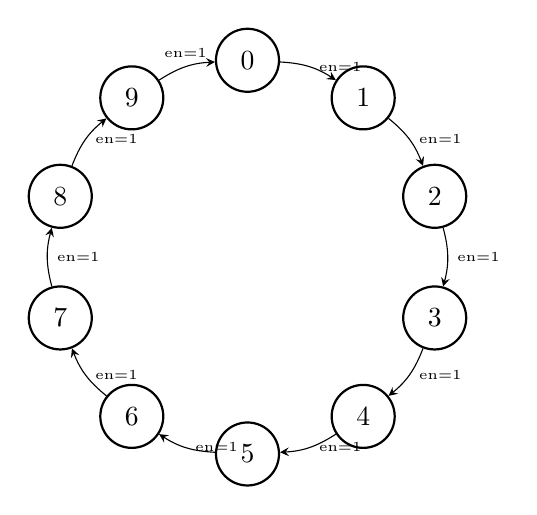
\begin{tikzpicture}[
  ->, >=stealth, auto, node distance=2.5cm,
  state/.style={circle, draw=black, thick, minimum size=0.8cm, inner sep=0pt}
]

% 10 states arranged in a circle
\node[state] (s0)  at (90:2.5)  {0};
\node[state] (s1)  at (54:2.5)  {1};
\node[state] (s2)  at (18:2.5)  {2};
\node[state] (s3)  at (-18:2.5) {3};
\node[state] (s4)  at (-54:2.5) {4};
\node[state] (s5)  at (-90:2.5) {5};
\node[state] (s6)  at (-126:2.5){6};
\node[state] (s7)  at (-162:2.5){7};
\node[state] (s8)  at (-198:2.5){8};
\node[state] (s9)  at (126:2.5) {9};

% Transitions en=1
\path (s0) edge[bend left=15] node[right, font=\tiny]{en=1} (s1);
\path (s1) edge[bend left=15] node[right, font=\tiny]{en=1} (s2);
\path (s2) edge[bend left=15] node[right, font=\tiny]{en=1} (s3);
\path (s3) edge[bend left=15] node[right, font=\tiny]{en=1} (s4);
\path (s4) edge[bend left=15] node[right, font=\tiny]{en=1} (s5);
\path (s5) edge[bend left=15] node[right, font=\tiny]{en=1} (s6);
\path (s6) edge[bend left=15] node[right, font=\tiny]{en=1} (s7);
\path (s7) edge[bend left=15] node[right, font=\tiny]{en=1} (s8);
\path (s8) edge[bend left=15] node[right, font=\tiny]{en=1} (s9);
\path (s9) edge[bend left=15] node[above, font=\tiny]{en=1} (s0);

\end{tikzpicture}
\end{center}

\noindent\textbf{状态说明：}
\begin{itemize}
  \item 共10个状态（S0--S9），对应计数值0--9
  \item \texttt{rst='1'} 时：任何状态同步复位到 S0（clk上升沿生效）
  \item \texttt{en='1'} 且 \texttt{rst='0'} 时：状态递增（S0$\rightarrow$S1$\rightarrow\cdots\rightarrow$S9$\rightarrow$S0）
  \item \texttt{en='0'} 且 \texttt{rst='0'} 时：状态保持不变
  \item \texttt{cout='1'}：当且仅当当前状态为S9（q=9）且 \texttt{en='1'} 时，\texttt{cout='1'}（组合逻辑输出）
\end{itemize}

\subsubsection*{(2) 模10计数器VHDL代码（10分）}

\begin{lstlisting}[caption={模10计数器——完整VHDL代码}, label={lst:ans04_mod10}]
library ieee;
use ieee.std_logic_1164.all;
use ieee.numeric_std.all;

entity mod10_counter is
  port (
    clk  : in  std_logic;                       -- 时钟信号
    rst  : in  std_logic;                       -- 同步清零（高有效）
    en   : in  std_logic;                       -- 计数使能（高有效）
    q    : out std_logic_vector(3 downto 0);    -- 当前计数值 (0~9)
    cout : out std_logic                        -- 进位输出（q=9且en=1时为1）
  );
end mod10_counter;

architecture rtl of mod10_counter is
  signal count : unsigned(3 downto 0);  -- 内部计数值
begin

  -- 同步计数进程
  count_proc: process(clk)
  begin
    if rising_edge(clk) then
      if rst = '1' then
        count <= (others => '0');        -- 同步清零
      elsif en = '1' then
        if count = 9 then
          count <= (others => '0');      -- 计到9回0
        else
          count <= count + 1;            -- 正常加1
        end if;
      end if;
    end if;
  end process;

  -- 输出赋值
  q <= std_logic_vector(count);

  -- 进位输出：组合逻辑，当前为9且使能有效时输出1
  cout <= '1' when (count = 9 and en = '1') else '0';

end rtl;
\end{lstlisting}

\noindent\textbf{关键设计要点：}
\begin{itemize}
  \item 采用\texttt{unsigned}类型作为内部计数器（需引用\texttt{ieee.numeric\_std.all}），便于算术运算。
  \item 同步清零在时钟上升沿检测\texttt{rst='1'}时生效，符合题目要求。
  \item \texttt{cout}为组合逻辑输出，仅在\texttt{count=9}且\texttt{en='1'}时为高，表示即将产生进位。
  \item 计数范围0--9，下一个时钟沿回到0（模10）。
\end{itemize}

\subsubsection*{(3) 模60计数器扩展VHDL代码（5分）}

\begin{lstlisting}[caption={模60计数器（0--59）——扩展代码}, label={lst:ans04_mod60}]
library ieee;
use ieee.std_logic_1164.all;
use ieee.numeric_std.all;

entity mod60_counter is
  port (
    clk  : in  std_logic;                       -- 时钟信号
    rst  : in  std_logic;                       -- 同步清零（高有效）
    en   : in  std_logic;                       -- 计数使能（高有效）
    q    : out std_logic_vector(5 downto 0);    -- 当前计数值 (0~59)，6位足够
    cout : out std_logic                        -- 进位输出（q=59且en=1时为1）
  );
end mod60_counter;

architecture rtl of mod60_counter is
  -- 关键改动：分为个位和十位两个计数器
  signal units : unsigned(3 downto 0);  -- 个位计数器 (0~9)
  signal tens  : unsigned(3 downto 0);  -- 十位计数器 (0~5)
begin

  count_proc: process(clk)
  begin
    if rising_edge(clk) then
      if rst = '1' then
        -- 同步清零：个位和十位均清零
        units <= (others => '0');
        tens  <= (others => '0');
      elsif en = '1' then
        -- ===== 关键改动：级联计数逻辑 =====
        if units = 9 then
          units <= (others => '0');      -- 个位回0
          if tens = 5 then
            tens <= (others => '0');     -- 十位计到5也回0（整体59->0）
          else
            tens <= tens + 1;            -- 十位加1
          end if;
        else
          units <= units + 1;            -- 个位正常加1
        end if;
      end if;
    end if;
  end process;

  -- 输出：合并个位和十位为6位宽计数值
  q(3 downto 0) <= std_logic_vector(units);
  q(5 downto 4) <= std_logic_vector(tens(1 downto 0));

  -- 进位输出：计数到最大值59且使能有效时输出1
  cout <= '1' when (units = 9 and tens = 5 and en = '1') else '0';

end rtl;
\end{lstlisting}

\noindent\textbf{关键改动说明：}
\begin{enumerate}
  \item \textbf{两级计数器结构：}将单个4位计数器拆分为个位（\texttt{units}, 0--9）和十位（\texttt{tens}, 0--5）两个子计数器。
  \item \textbf{级联进位逻辑：}当个位计到9时，个位清零并向十位发出进位；当十位计到5且个位为9时，十位也清零（整体回到0）。
  \item \textbf{输出合并：}将个位（4位）和十位（2位）拼接为6位输出\texttt{q[5:0]}。
  \item \textbf{进位条件修改：}\texttt{cout}的条件从\texttt{count=9}变为\texttt{units=9 and tens=5}（即整体计数值为59）。
  \item \textbf{位宽变化：}输出\texttt{q}从4位扩展到6位（足够表示0--59）。
\end{enumerate}

%-----------------------------------------------------------------------------
\subsection*{设计题3：Moore型``101''序列检测器（20分）}
%-----------------------------------------------------------------------------

\begin{framed}
\textbf{评分标准：}
\begin{itemize}
  \item 状态转移图（6分）：状态定义完整2分，转移条件和输出标注正确3分，图面规范1分。
  \item 状态转移表（4分）：表格完整2分（含现态、输入、次态、输出），编码合理1分，与状态图一致1分。
  \item VHDL代码（10分）：状态类型定义与编码2分，状态寄存器进程2分，次态逻辑进程3分，输出逻辑进程2分，重叠检测正确1分。
\end{itemize}
\end{framed}

\subsubsection*{(1) 状态转移图（6分）}

\begin{center}
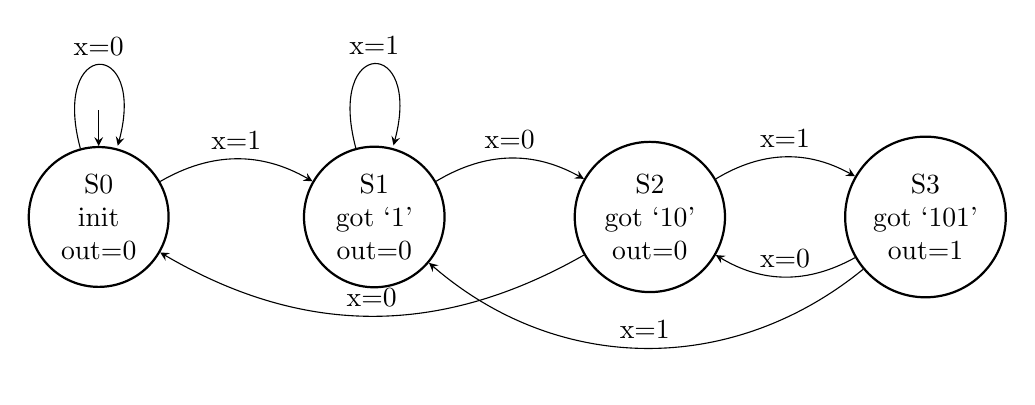
\begin{tikzpicture}[
  ->, >=stealth, auto, node distance=3.5cm,
  every state/.style={draw=black, thick, minimum size=1.2cm, align=center}
]

% S0: initial / no match
\node[state, initial above, initial text=] (S0) {S0\\init\\out=0};

% S1: got '1'
\node[state, right of=S0] (S1) {S1\\got `1'\\out=0};

% S2: got '10'
\node[state, right of=S1] (S2) {S2\\got `10'\\out=0};

% S3: got '101' -> detect!
\node[state, right of=S2] (S3) {S3\\got `101'\\out=1};

% Transitions
\path (S0) edge[loop above]   node {x=0} (S0);
\path (S0) edge[bend left]    node[above] {x=1} (S1);

\path (S1) edge[loop above]   node {x=1} (S1);
\path (S1) edge[bend left]    node[above] {x=0} (S2);

\path (S2) edge[bend left]    node[above] {x=0} (S0);
\path (S2) edge[bend left]    node[above] {x=1} (S3);

\path (S3) edge[bend left=40] node[above] {x=1} (S1);
\path (S3) edge[bend left]    node[above] {x=0} (S2);

\end{tikzpicture}
\end{center}

\noindent\textbf{状态定义与转移说明：}
\begin{itemize}
  \item \textbf{S0（初始状态，output=0）：}尚未检测到有效序列。\texttt{x=0}保持S0；\texttt{x=1}进入S1。
  \item \textbf{S1（已匹配`1'，output=0）：}检测到一个`1'。\texttt{x=1}保持S1（新`1'重新开始）；\texttt{x=0}进入S2。
  \item \textbf{S2（已匹配`10'，output=0）：}检测到`10'。\texttt{x=1}进入S3（完成`101'）；\texttt{x=0}回到S0（连续两个0无效）。
  \item \textbf{S3（已匹配`101'，output=1）：}成功检测到`101'序列。\texttt{x=1}进入S1（重叠检测：最后一个`1'可作新序列开始）；\texttt{x=0}进入S2（重叠检测：最后`10'可作新序列前缀）。
\end{itemize}

\noindent\textbf{重叠检测示例（\texttt{10101}）：}
\begin{center}
\begin{tabular}{c|ccccc}
输入序列 & 1 & 0 & 1 & 0 & 1 \\
\hline
状态变化 & S0$\rightarrow$S1$\rightarrow$S2$\rightarrow$S3$\rightarrow$S2$\rightarrow$S3 \\
输出 & 0 & 0 & 1 & 0 & 1 \\
\end{tabular}
\end{center}
可见\texttt{10101}确实检测到了两次\texttt{101}（位置1--3和位置3--5共享中间的`1'）。

\subsubsection*{(2) 状态转移表（4分）}

\begin{center}
\textbf{状态编码：} S0=``00'', S1=``01'', S2=``10'', S3=``11''

\vspace{0.3cm}
\begin{tabular}{|c|c|c|c|}
\hline
\textbf{现态（PS）} & \textbf{输入 x} & \textbf{次态（NS）} & \textbf{输出（detect）} \\
\hline
S0 (00) & 0 & S0 (00) & 0 \\
S0 (00) & 1 & S1 (01) & 0 \\
\hline
S1 (01) & 0 & S2 (10) & 0 \\
S1 (01) & 1 & S1 (01) & 0 \\
\hline
S2 (10) & 0 & S0 (00) & 0 \\
S2 (10) & 1 & S3 (11) & 0 \\
\hline
S3 (11) & 0 & S2 (10) & 1 \\
S3 (11) & 1 & S1 (01) & 1 \\
\hline
\end{tabular}
\end{center}

\noindent\textbf{说明：}Moore型状态机的输出仅取决于当前状态。从表中可见，仅当现态为S3时输出\texttt{detect=1}，其余状态输出为0。

\subsubsection*{(3) 完整VHDL代码——三进程描述风格（10分）}

\begin{lstlisting}[caption={Moore型``101''序列检测器——三进程描述}, label={lst:ans04_fsm}]
library ieee;
use ieee.std_logic_1164.all;

entity seq_detector_101 is
  port (
    clk    : in  std_logic;              -- 时钟信号
    rst    : in  std_logic;              -- 同步复位（高有效）
    x      : in  std_logic;              -- 串行输入数据
    detect : out std_logic               -- 检测输出（Moore型）
  );
end seq_detector_101;

architecture moore_3proc of seq_detector_101 is

  -- 状态类型定义：使用枚举类型，代码清晰可读
  type state_type is (S0, S1, S2, S3);
  signal current_state, next_state : state_type;

begin

  -- ========================================================
  -- 进程1：状态寄存器（同步时序逻辑）
  -- 功能：在时钟上升沿完成状态切换，处理同步复位
  -- ========================================================
  state_reg: process(clk)
  begin
    if rising_edge(clk) then
      if rst = '1' then
        current_state <= S0;              -- 同步复位到初始态
      else
        current_state <= next_state;      -- 正常状态转移
      end if;
    end if;
  end process;

  -- ========================================================
  -- 进程2：次态逻辑（组合逻辑）
  -- 功能：根据当前状态和输入决定下一个状态
  -- 关键：正确处理重叠检测的转移路径
  -- ========================================================
  next_state_logic: process(current_state, x)
  begin
    -- 默认值（防止锁存器）
    next_state <= S0;

    case current_state is
      when S0 =>                         -- 初始状态
        if x = '0' then
          next_state <= S0;
        else
          next_state <= S1;              -- x=1: 进入S1
        end if;

      when S1 =>                         -- 已匹配 '1'
        if x = '0' then
          next_state <= S2;              -- x=0: 获得"10"
        else
          next_state <= S1;              -- x=1: 保留在S1
        end if;

      when S2 =>                         -- 已匹配 '10'
        if x = '0' then
          next_state <= S0;              -- x=0: 回到初始
        else
          next_state <= S3;              -- x=1: 完成"101"
        end if;

      when S3 =>                         -- 已匹配 '101'（检测成功）
        if x = '0' then
          next_state <= S2;   -- 重叠: 最后"10"可作新前缀
        else
          next_state <= S1;   -- 重叠: 最后"1"可作新开始
        end if;

      when others =>
        next_state <= S0;                -- 安全默认
    end case;
  end process;

  -- ========================================================
  -- 进程3：输出逻辑（组合逻辑）
  -- Moore型：输出仅取决于当前状态
  -- ========================================================
  output_logic: process(current_state)
  begin
    case current_state is
      when S3 =>
        detect <= '1';                   -- 仅S3状态下输出1
      when others =>
        detect <= '0';
    end case;
  end process;

end moore_3proc;
\end{lstlisting}

\noindent\textbf{设计说明：}
\begin{itemize}
  \item \textbf{三进程风格：}将状态寄存器、次态逻辑、输出逻辑分别放在三个独立进程中，结构清晰、易于维护。
  \item \textbf{状态编码：}使用VHDL枚举类型（\texttt{state\_type}），综合工具自动进行状态编码（one-hot、binary等由综合选项控制），代码可读性高。
  \item \textbf{Moore型特征：}输出\texttt{detect}仅由\texttt{current\_state}决定（进程3的敏感表中不含\texttt{x}），与输入\texttt{x}无关。这确保了输出在一个完整的时钟周期内保持稳定。
  \item \textbf{重叠检测：}S3状态的转移路径是核心——\texttt{x=0}时返回S2（利用`10'前缀），\texttt{x=1}时返回S1（利用`1'前缀），确保\texttt{10101}能检测出两次匹配。
  \item \textbf{同步复位：}\texttt{rst}高有效，仅在时钟上升沿检测，符合题目要求。
\end{itemize}

%=============================================================================
\section*{本套试卷评分汇总}
%=============================================================================

\begin{center}
\begin{tabular}{|l|c|c|}
\hline
\textbf{题型} & \textbf{题号/内容} & \textbf{分值} \\
\hline
一、选择题   & 第1--6题 & 18分 \\
二、填空题   & 第1--4题 & 12分 \\
三、程序改错 & 6处错误找5处满分 & 5分 \\
四、程序阅读 & 优先级编码器分析 & 5分 \\
五、设计题1  & 8位比较器（框图+VHDL+TB） & 20分 \\
五、设计题2  & 模10/模60计数器 & 20分 \\
五、设计题3  & Moore型``101''检测器 & 20分 \\
\hline
\textbf{合计} & & \textbf{100分} \\
\hline
\end{tabular}
\end{center}
